\section{Clasificador}

\subsection{Metodología}
\begin{frame}
    \frametitle{Metodología}

    \begin{itemize}
        \item Se utilizan SVM, kNN, DT, GNB y MNB.
        \item Se divide en 80\% entrenamiento y 20\% evaluación.
        \item Se usa validación cruzada sobre el conjunto de entrenamiento para resultados intermedios durante el desarollo y el conjunto de evaluación para el resultado final.
    \end{itemize}
\end{frame}
\note{
    Se usa el conjunto de evaluación al final para no sesgarse demasiado a los resultados.
}

\subsection{Línea base}
\begin{frame}[allowframebreaks]
    \frametitle{Línea base}

    \begin{enumerate}
        \item BoW + MNB

        \item Clasificador que predice según lo que dice la mayoría (Negativo)
    \end{enumerate}

    \begin{center}
        \scriptsize
        \begin{tabular}{ c | r | r | r | r | r | r | r }
            & \multicolumn{1}{c |}{Precisión} & \multicolumn{1}{c |}{Recall} & \multicolumn{1}{c |}{$F_1$} & \multicolumn{1}{c |}{Prec. neg.} & \multicolumn{1}{c |}{Rec. neg.} & \multicolumn{1}{c |}{$F_1$ neg.} & \multicolumn{1}{c}{Acierto} \\
            \hline
            LB1 & 65,15 & 82,71 & 72,89 & 96,33 & 91,19 & 93,65 & 89,71 \\
            \hline
            LB2 & indef. & 0,00 & indef. & 82,49 & 100,00 & 90,41 & 82,49 \\
        \end{tabular}
    \end{center}
\end{frame}

\subsection{Características}

\begin{frame}
    \frametitle{Qué se busca}

    \begin{itemize}
        \item Contradicción y negatividad
        \item Formato e informalidad
        \item Orientación en personas
        \item Temas recurrentes en chistes
    \end{itemize}
\end{frame}

\begin{frame}
    \frametitle{Presencia de animales}

    \begin{itemize}
        \item Se conforma una lista de animales a partir de los chistes de animales de Chistes.com ($DIC_A$)
        \item Intersección de multiconjuntos:
    \end{itemize}

    \begin{center}
        \[
            PresenciaAnimales(tweet) = \frac{|tweet \cap DIC_A|}{\sqrt{|tweet|}}
        \]
    \end{center}
\end{frame}
\note{
    Características simples.
    $tweet$ es visto como una lista de tokens.
    En general todas las featuers se normalizan según el largo del tweet en tokens, para no sesgar.
}

\begin{frame}
    \frametitle{Jerga sexual}

    \begin{itemize}
        \item Se arma un diccionario de jerga sexual mediante \emph{Bootstrapping} en Twitter.
        \item Intersección de multiconjuntos:
    \end{itemize}

    \begin{center}
        \[
            JergaSexual(tweet) = \frac{|tweet \cap DIC_{JS}|}{\sqrt{|tweet|}}
        \]
    \end{center}
\end{frame}

\begin{frame}
    \frametitle{Primera persona}

    \begin{itemize}
        \item Se busca por palabras flexionadas en primera persona
    \end{itemize}
\end{frame}

\begin{frame}
    \frametitle{Segunda persona}

    \begin{itemize}
        \item Se busca por palabras flexionadas en segunda persona
    \end{itemize}
\end{frame}

\begin{frame}
    \frametitle{Distancia temática}

    \begin{itemize}
        \item Cercanía a un chiste de Chistes.com o cercanía a una oración de la Wikipedia.
        \item BoW + MNB
        \item Categorías
        \begin{itemize}
            \item Chistes cortos
            \item Adivinanzas
            \item Animales
            \item Atlantes
            \item Otros...
        \end{itemize}
    \end{itemize}
\end{frame}
\note{TODO: Aclarar qué es atlantes.}

\begin{frame}
    \frametitle{Diálogo}

    \begin{itemize}
        \item Si el tweet es un diálogo o no
    \end{itemize}
\end{frame}

\begin{frame}
    \frametitle{Preguntas-respuestas}

    \begin{itemize}
        \item Cantidad de preguntas seguidas de respuestas en el tweet.
    \end{itemize}
\end{frame}

\begin{frame}
    \frametitle{Palabras clave}

    \begin{itemize}
        \item Lista de palabras frecuentes en tweets
        \item Intersección de multiconjuntos:
    \end{itemize}

    \begin{center}
        \[
            PalabrasClave(tweet) = \frac{|tweet \cap DIC_{PF}|}{\sqrt{|tweet|}}
        \]
    \end{center}
\end{frame}

\begin{frame}
    \frametitle{Links}

    \begin{itemize}
        \item Cantidad de hipervínculos en el tweet
    \end{itemize}
\end{frame}

\begin{frame}
    \frametitle{Antónimos}

    \begin{itemize}
        \item Cantidad de pares de antónimos en el tweet:
    \end{itemize}

    \begin{center}
        \[
            Antonimos(tweet) = \frac{|\{pares\ de\ antonimos\}|}{\sqrt{|tweet|}}
        \]
    \end{center}
\end{frame}

\begin{frame}
    \frametitle{Hashtags}

    \begin{itemize}
        \item Cantidad de hashtags en el tweet
    \end{itemize}
\end{frame}

\begin{frame}
    \frametitle{Exclamación}

    \begin{itemize}
        \item Cantidad de signos de exclamación:
    \end{itemize}

    \begin{center}
        \[
            Exclamacion(tweet) = \frac{|\{signos\ de\ exclamacion\}|}{\sqrt{|tweet|}}
        \]
    \end{center}
\end{frame}

\begin{frame}
    \frametitle{Exclamación}

    \begin{itemize}
        \item Cantidad de palabras totalmente en mayúsculas:
    \end{itemize}

    \begin{center}
        \[
            PalabrasMayusculas(tweet) = \frac{|\{palabras\ mayusculas\}|}{\sqrt{|tweet|}}
        \]
    \end{center}
\end{frame}

\begin{frame}
    \frametitle{Negación}

    \begin{itemize}
        \item Cantidad de ``no'' en el tweet
    \end{itemize}
\end{frame}

\begin{frame}
    \frametitle{Palabras fuera del vocabluario (OOV)}

    \begin{itemize}
        \item Cantidad de palabras fuera del vocabulario, dividiento entre el total
        \item Son varias características:
        \begin{itemize}
            \item Freeling
            \item Freeling-Google
            \item Freeling-Wiktionary
            \item Wiktionary
        \end{itemize}
    \end{itemize}
\end{frame}
\note{
    Las distintas combinaciones de vocabulario debido a costo de uso y debido a ventajas y desventajas de cada uno. \textbf{Freeling} el más barato de usar, offline. Tiene un español más clasico, pero no tiene palabras ``nuevas''. \textbf{Wiktionary} tiene un término medio de todo. Es online, pero no limita su uso. Con \textbf{Google} se pueden obtener muchas palabras ``nuevas'' (como iPhone) y también detección de errores ortográficos, pero limita su uso.
}

\begin{frame}
    \frametitle{Palabras no españolas}

    \begin{itemize}
        \item Cantidad de palabras que tienen caracteres fuera del alfabeto español, normalizado según el total.
    \end{itemize}
\end{frame}

\subsection{Selección de características}
\begin{frame}[allowframebreaks]
    \frametitle{Selección de características}

    \begin{itemize}
        \item Se utiliza la Eliminación recursiva de atributos para seleccionar aquellos relevantes y no redundantes.
        \item Se descartan Negación, Palabras no españolas y Antónimos
    \end{itemize}

    \begin{center}
        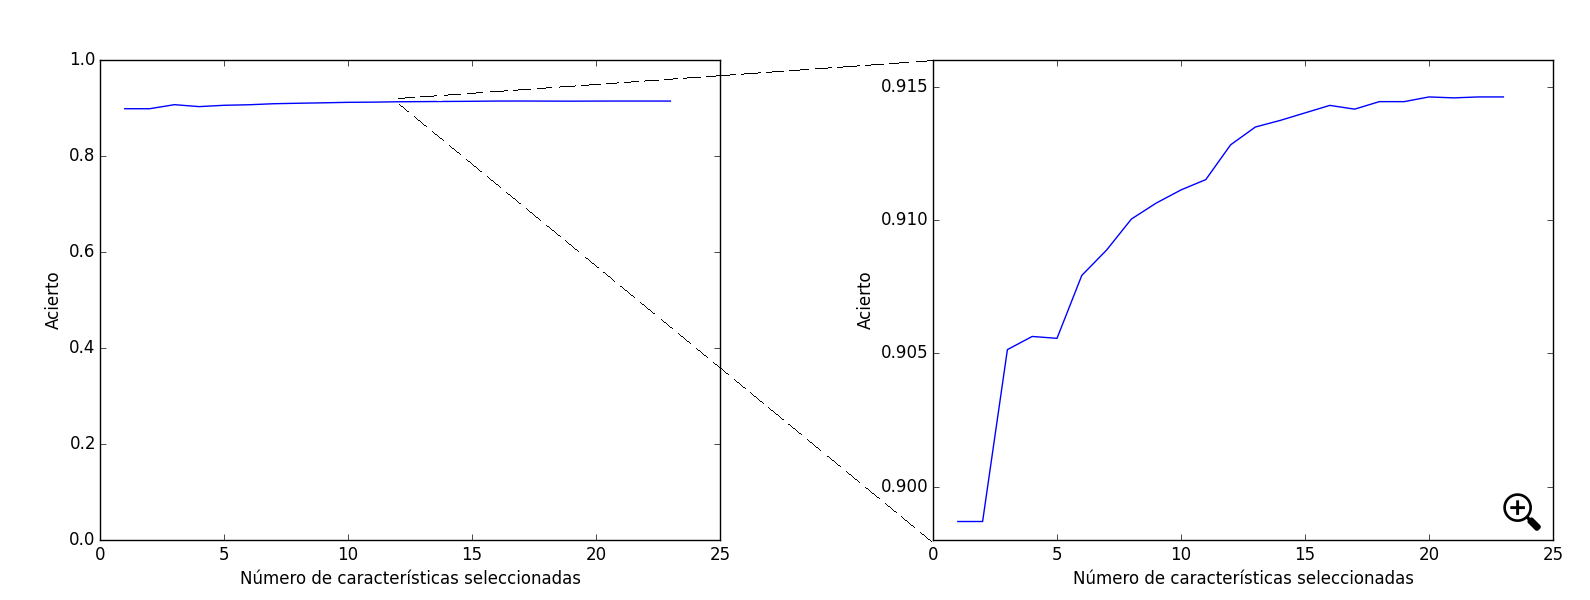
\includegraphics{rfe.png}
    \end{center}
\end{frame}

\subsection{Resultados obtenidos}
\begin{frame}
    \frametitle{Resultados obtenidos}

    \begin{center}
        \scriptsize

        \begin{tabular}{ c | r | r | r | r | r | r | r }
            & \multicolumn{1}{c |}{Precisión} & \multicolumn{1}{c |}{Recall} & \multicolumn{1}{c |}{$F_1$} & \multicolumn{1}{c |}{Prec. neg.} & \multicolumn{1}{c |}{Rec. neg.} & \multicolumn{1}{c |}{$F_1$ neg.} & \multicolumn{1}{c}{Acierto} \\
            \hline
            LB1 & 61,68 & \textbf{84,63} & 71,35 & \textbf{96,59} & 89,23 & 71,35 & 88,45 \\
            \hline
            LB2 & indef. & 0,00 & indef. & 83,00 & \textbf{100,00} & 90,71 & 83,00 \\
            \hline
            SVM & \textbf{83,61} & 68,85 & \textbf{75,52} & 93,84 & 97,24 & \textbf{95,51} & \textbf{92,45} \\
            \hline
            DT & 66,51 & 67,54 & 67,02 & 93,33 & 93,03 & 93,18 & 88,85 \\
            \hline
            GNB & 57,49 & \textbf{78,17} & 66,25 & \textbf{95,17} & 88,16 & 91,53 & 86,46 \\
            \hline
            MNB & 84,76 & 60,02 & 70,27 & 92,27 & \textbf{97,79} & 94,95 & 91,37 \\
            \hline
            KNN & 81,26 & 66,31 & 73,03 & 93,35 & 96,87 & 95,08 & 91,67 \\
        \end{tabular}

        \vfill

        \begin{tabular}{ c | r | r }
            \textbf{son/clasif.} & Positivos & Negativos \\
            \hline
            Positivos & 842 & 381 \\
            \hline
            Negativos & 165 & 5805 \\
        \end{tabular}
    \end{center}
\end{frame}
\note{TODO: decir que es luego del escalado y demás}

\subsection{Otros análisis}

\subsubsection{Evaluación en el conjunto de entrenamiento}
\begin{frame}
    \frametitle{Evaluación en el conjunto de entrenamiento}

    \begin{itemize}
        \item Es una ``cota superior''
    \end{itemize}

    \begin{center}
        \scriptsize
        \begin{tabular}{ c | r | r | r | r | r | r | r }
            & \multicolumn{1}{c |}{Precisión} & \multicolumn{1}{c |}{Recall} & \multicolumn{1}{c |}{$F_1$} & \multicolumn{1}{c |}{Prec. neg.} & \multicolumn{1}{c |}{Rec. neg.} & \multicolumn{1}{c |}{$F_1$ neg.} & \multicolumn{1}{c}{Acierto} \\
            \hline
            SVM & 87,46 & 69,61 & 77,52 & 94,16 & 98,01 & 96,05 & 93,28 \\
            \hline
            DT & \textbf{99,96} & \textbf{98,82} & \textbf{99,38} & \textbf{99,76} & \textbf{99,99} & \textbf{99,88} & \textbf{99,80} \\
            \hline
            GNB & 58,06 & 77,65 & 66,44 & 95,21 & 88,79 & 91,89 & 86,94 \\
            \hline
            MNB & 84,56 & 58,93 & 69,46 & 92,26 & 97,85 & 94,97 & 91,67 \\
            \hline
            KNN & 86,98 & 71,47 & 78,47 & 94,49 & 97,86 & 96,15 & 93,47 \\
        \end{tabular}
    \end{center}
\end{frame}

\begin{frame}
    \frametitle{Evaluación en el conjunto de entrenamiento II}

    \begin{itemize}
        \item ¿Por qué DT no da 100\%? Debería darlo.
        \item Las características no discriminan completamente a la clase.
        \item ¿Hay errores en el corpus?
    \end{itemize}
\end{frame}

\begin{frame}[allowframebreaks]
    \frametitle{Inconsistencias en el corpus}

    \begin{itemize}
        \item Siguiendo la distancia mínima de edición en tweets (la granularidad es una palabra): se encontraron 367 pares de tweets ``parecidos'' pero con distinto valor de la clase objetivo.
    \end{itemize}

    \begin{example}
        Limpiar tu cuarto = 1\% limpieza. 30\% quejarse. 69\% jugar con lo que vas encontrando.
    \end{example}

    \begin{example}
        Limpiar tu cuarto:

        1\% limpieza.

        30\% quejarse.

        69\% jugar con lo que vas encontrando.
    \end{example}

    \note{
        En el primer caso son casi las mismas palabras, pero distinto espaciado y puntuación.
    }

    \framebreak

    \begin{itemize}
        \item Luego se buscan aquellos con mismos valores de atributos pero distinta clase: 30 pares encontrados.
    \end{itemize}

    \begin{example}
        \#TerminarUnaNotaDeSuicidioCon Soy Darks.
    \end{example}

    \begin{example}
        \#SiYoMeLlamaraKevinRoldan Me suicidaria.
    \end{example}
\end{frame}

\begin{frame}
    \frametitle{Inconsistencias en el corpus III}

    \begin{itemize}
        \item Hay inconsistencias en la anotación (era esperado)
        \item Hay una mejora sobre el corpus de entrenamiento quitando estas instancias:

        \begin{center}
            \scriptsize
            \begin{tabular}{ c | r | r | r | r | r | r | r }
                \textbf{SVM} & \multicolumn{1}{c |}{Precisión} & \multicolumn{1}{c |}{Recall} & \multicolumn{1}{c |}{$F_1$} & \multicolumn{1}{c |}{Prec. neg.} & \multicolumn{1}{c |}{Rec. neg.} & \multicolumn{1}{c |}{$F_1$ neg.} & \multicolumn{1}{c}{Acierto} \\
                \hline
                Antes & 87,46 & 69,61 & 77,52 & 94,16 & 98,01 & 96,05 & 93,28 \\
                \hline
                Después & 88,96 & 71,27 & 79,13 & 94,72 & 98,31 & 96,48 & 93,98 \\
            \end{tabular}
        \end{center}
    \end{itemize}

    \begin{itemize}
        \item Y en el de corpus de evaluación:

        \begin{center}
            \scriptsize
             \begin{tabular}{ c | r | r | r | r | r | r | r }
                \textbf{SVM} & \multicolumn{1}{c |}{Precisión} & \multicolumn{1}{c |}{Recall} & \multicolumn{1}{c |}{$F_1$} & \multicolumn{1}{c |}{Prec. neg.} & \multicolumn{1}{c |}{Rec. neg.} & \multicolumn{1}{c |}{$F_1$ neg.} & \multicolumn{1}{c}{Acierto} \\
                \hline
                Antes & 83,61 & 68,85 & 75,52 & 93,84 & 97,24 & 95,51 & 92,45 \\
                \hline
                Después & 85,71 & 69,21 & 76,58 & 94,20 & 97,75 & 95,94 & 93,08 \\
            \end{tabular}
        \end{center}
    \end{itemize}
\end{frame}

\subsubsection{Tweets censurados}
\begin{frame}
    \frametitle{Tweets censurados}

    \begin{itemize}
        \item El clasificador está sesgado a no conocer los tweets con contenido explícito
        \item Se anotan a mano los 303 tweets censurados y se agregan
        \item Hay una pequeña mejora:
        \begin{center}
            \scriptsize
            \begin{tabular}{ c | r | r | r | r | r | r | r }
                \textbf{SVM} & \multicolumn{1}{c |}{Precisión} & \multicolumn{1}{c |}{Recall} & \multicolumn{1}{c |}{$F_1$} & \multicolumn{1}{c |}{Prec. neg.} & \multicolumn{1}{c |}{Rec. neg.} & \multicolumn{1}{c |}{$F_1$ neg.} & \multicolumn{1}{c}{Acierto} \\
                \hline
                Antes & 83,61 & 68,85 & 75,52 & 93,84 & 97,24 & 95,51 & 92,45 \\
                \hline
                Después & 84,01 & 69,59 & 76,13 & 93,74 & 97,17 & 95,43 & 92,32 \\
            \end{tabular}
        \end{center}
        \item Un nuevo estudio de importancia de las características revela que no varía Jerga sexual: se agrega más variedad que jerga sexual.
    \end{itemize}
\end{frame}

\subsubsection{Restricción a cuentas humorísticas}
\begin{frame}
    \frametitle{Restricción a cuentas humorísticas}

    \begin{itemize}
        \item Es una tarea más difícil
        \item Igualmente se logran buenos resultados:

        \begin{center}
            \scriptsize
            \begin{tabular}{ c | r | r | r | r | r | r | r }
                & \multicolumn{1}{c |}{Precisión} & \multicolumn{1}{c |}{Recall} & \multicolumn{1}{c |}{$F_1$} & \multicolumn{1}{c |}{Prec. neg.} & \multicolumn{1}{c |}{Rec. neg.} & \multicolumn{1}{c |}{$F_1$ neg.} & \multicolumn{1}{c}{Acierto} \\
                \hline
                SVM & \textbf{81,87} & 73,83 & 77,64 & 78,47 & \textbf{85,36} & \textbf{81,77} & \textbf{79,92} \\
                \hline
                DT & 74,49 & 75,48 & 74,98 & 72,20 & 71,14 & 71,66 & 74,12 \\
                \hline
                GNB & 78,72 & 78,55 & \textbf{78,64} & 76,10 & 76,29 & 76,19 & 77,48 \\
                \hline
                MNB & 68,52 & \textbf{85,45} & 76,06 & \textbf{83,27} & 64,86 & 72,9 & 74,58 \\
                \hline
                KNN & 79,24 & 73,02 & 76,00 & 77,43 & 82,87 & 80,06 & 78,14 \\
            \end{tabular}
        \end{center}
    \end{itemize}
\end{frame}

\begin{frame}
    \frametitle{Métricas ponderadas según calificación}

    \begin{itemize}
        \item Tiene sentido sólo para los tweets que tuvieron votos y para la medida recall
        \item Promedio de estrellas, $PE_t = \frac{\sum_{i = 1}^{5} i \times v_{ti}}{v_t}$
        \item $recall_{ponderado} = \frac{\sum_{t \in VP} PE_t} {\sum_{t \in VP} PE_t + \sum_{t \in FN} PE_t} = 70.68\%$
        \item $\frac{recall_{ponderado}}{recall} = \frac{prom_{VP}}{prom_H} = 1.0266$
        \item Hay un (muy) leve sesgo del clasificador SVM a dar como positivos aquellos tweets que tienen mayor promedio de estrellas.
        \item Matriz de confusión:

        \begin{center}
            \begin{tabular}{ c | r | r }
                \textbf{son/clasificados} & Humor & No humor \\
                \hline
                Humor & 2,7227 & 2,4961 \\
                \hline
                No humor & 0,0256 & 0,0300 \\
            \end{tabular}
        \end{center}
    \end{itemize}
\end{frame}

\subsubsection{Clasificación según categorías de cuentas no humorísticas}
\begin{frame}
    \frametitle{Clasificación según categorías de cuentas no humorísticas}

    \begin{center}
        \scriptsize
        \begin{tabular}{ c | r | r | r | r | r | r | r }
            \textbf{SVM} & \multicolumn{1}{c |}{Precisión} & \multicolumn{1}{c |}{Recall} & \multicolumn{1}{c |}{$F_1$} & \multicolumn{1}{c |}{Prec. neg.} & \multicolumn{1}{c |}{Rec. neg.} & \multicolumn{1}{c |}{$F_1$ neg.} & \multicolumn{1}{c}{Acierto} \\
            \hline
            Noticias & \textbf{97,00} & \textbf{95,18} & \textbf{96,08} & \textbf{96,95} & \textbf{98,12} & \textbf{97,53} & \textbf{96,97} \\
            \hline
            Reflexiones & 94,95 & 82,99 & 88,57 & 83,95 & 95,27 & 89,25 & 88,92 \\
            \hline
            Curiosidades & 94,64 & 83,73 & 88,85 & 88,24 & 96,26 & 92,08 & 90,74 \\
        \end{tabular}
    \end{center}
\end{frame}

\subsubsection{Tweets dusosos}
\begin{frame}
    \frametitle{Tweets dudosos}

    \begin{center}
        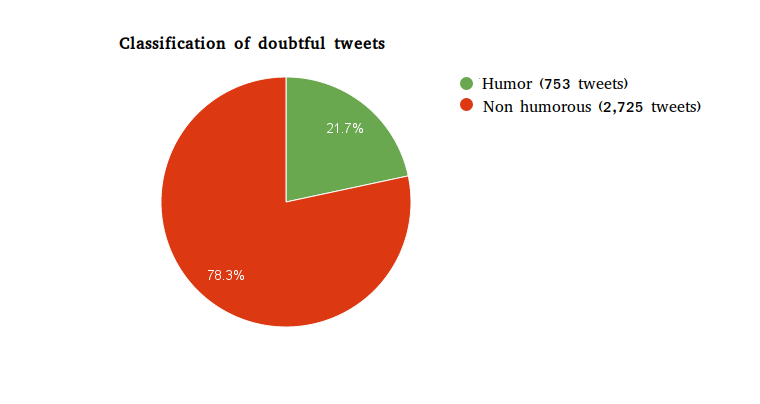
\includegraphics{dudosos.png}
    \end{center}
\end{frame}
